% TODO this would be the alternative to the table of toplogies in chapetr 2
% \begin{center}
%     \centering
% \begin{tabular}{|>{\centering\arraybackslash}m{2cm}|>{\centering\arraybackslash}m{4cm}|>{\arraybackslash}m{8.5cm}|}
% \hline
% \textbf{Name} & \textbf{Image} & \textbf{Description} \\
% \hline
% Centralized & 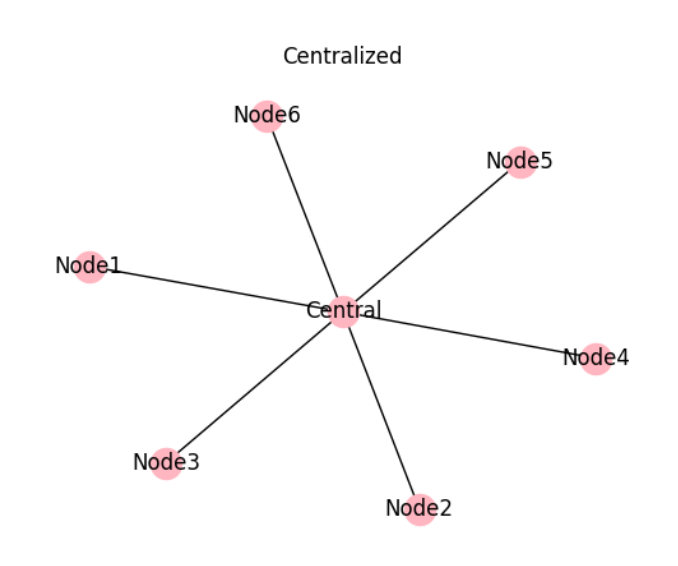
\includegraphics[width=4cm]{centralized.png} & The centralized topology is characterized by a strict hierarchical structure in which all nodes are connected with one central server that orchestrates them and performs the necessary steps for the combination of the machine learning. It serves a simple coordination but is limited in scalability due to having a single point of failure.\\
% \hline
% Tree & 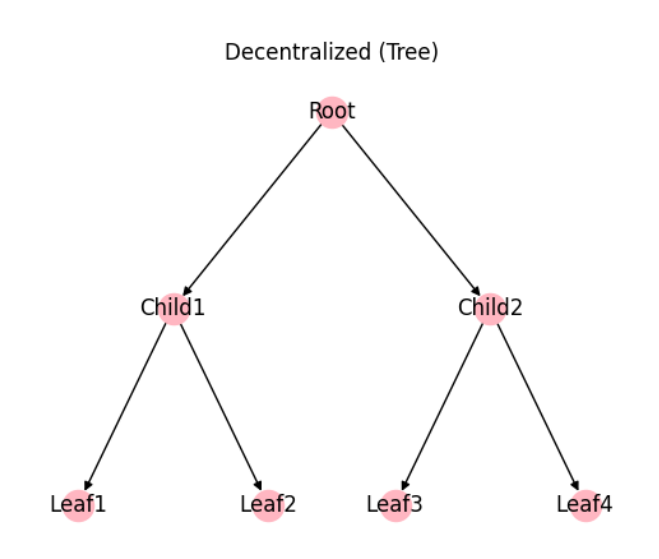
\includegraphics[width=4cm]{tree.png} & The tree topology is a decentralized topology in which the nodes are structured hierarchical. The communication takes place between the nodes in specific directions. Information is communicated upwards and distributed downwards. This is scalable as every node only communicates with children or parents. \\
% \hline
% Parameter Server & 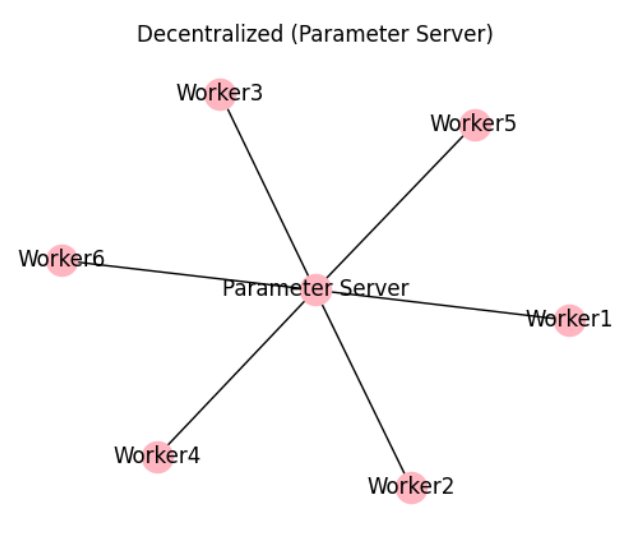
\includegraphics[width=4cm]{parameterserver.png} & This topology is a second decentralized topology that combines centralied parameter servers to store and retrieve gradients with decentralized \ac{ML} nodes. These servers have a shared memory, so the parameters can be synchronized between multiple parts. The disadvantage of this is that all communication happens at the parameter servers, creating bottlenecks if many workers are combined with few servers. \\
% \hline
% Fully Distributed & 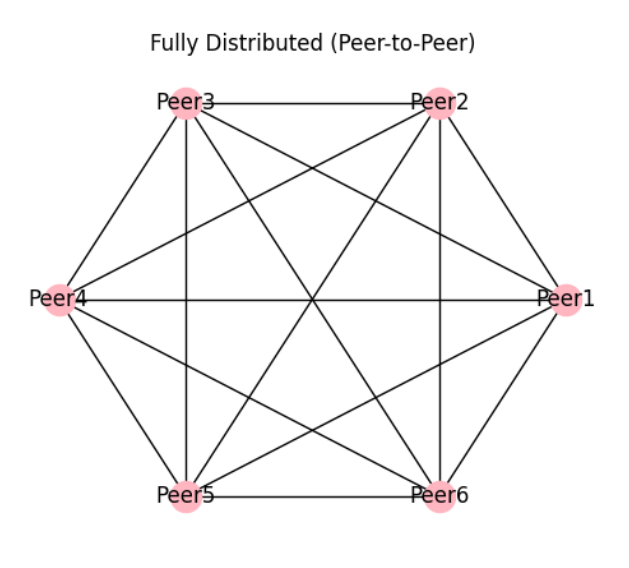
\includegraphics[width=4cm]{fullydistributed.png} & A fully distributed topology works like a peer-to-peer network, meaning each node holds its own copy of the models parameters and is able to communicate with all other nodes. Communciation is possible in every direction and at any time. This is very scalable, as new workers can be added without a high centralized overload, but it has the disadvantage that the communication can create a high overhead if every worker broadcasts its information. \\
% \hline
% \end{tabular}
% \end{center}